% !TEX program = lualatex
\documentclass[a4paper,13pt,3p,twoside]{report}

\usepackage[main=english,vietnamese]{babel}

\usepackage{fontspec}
\setmainfont{Times New Roman}
\usepackage[fontsize=13pt]{scrextend}
\usepackage[top=2cm, bottom=2cm, left=3.5cm, right=2.5cm]{geometry}

\usepackage{parskip}
\usepackage{indentfirst}
\usepackage{enumitem}
\usepackage{outlines}

\usepackage{float}
\usepackage{pdflscape}
\usepackage{graphicx}

\usepackage{appendix}
\usepackage{xcolor}

\usepackage{amsthm}
\usepackage{amsmath}
\usepackage{amssymb}
\usepackage{latexsym}
\usepackage{amsbsy}
\usepackage{array}
\usepackage{subfiles}
\usepackage{titlesec}
\usepackage{titletoc}
\usepackage{chngcntr}
\usepackage{afterpage}
\usepackage[ruled,vlined]{algorithm2e}
\usepackage{capt-of}
\usepackage{multirow}
\usepackage[font=small,labelfont=bf]{caption}

\usepackage{listings}
\usepackage{subcaption}

\usepackage[nonumberlist, nopostdot, nogroupskip, acronym]{glossaries}
\usepackage{glossary-superragged}
\setglossarystyle{superraggedheaderborder}
\usepackage{setspace}

\usepackage{blindtext}

\usepackage{csquotes}
\usepackage[backend=biber,style=ieee]{biblatex}

\addbibresource{reference.bib}

\def \TITLE{GRADUATION THESIS}
\def \AUTHOR{Nguyễn Trí Nghĩa}

\usepackage{fancyhdr}

\fancypagestyle{plain}{
  \fancyhf{}
  \fancyfoot[RO, RE]{\thepage}
  \renewcommand{\headrulewidth}{0pt}
  \renewcommand{\footrulewidth}{0pt}
}

\setlength{\headheight}{16pt}

\titleformat{\chapter}[hang]{\centering\bfseries}{CHAPTER \thechapter.}{5pt}{}
\titlespacing*{\chapter}{0pt}{-20pt}{20pt}

\titleformat{\section}[hang]{\bfseries}{\thechapter.\arabic{section}}{12pt}{}
\titlespacing{\section}{0pt}{\parskip}{0.5\parskip}

\titleformat{\subsection}[hang]{\bfseries}{\thechapter.\arabic{section}.\arabic{subsection}\ \ \ \ }{0pt}{}
\titlespacing{\subsection}{30pt}{\parskip}{0.5\parskip}

\renewcommand\thesubsubsection{\alph{subsubsection}}
\titleformat{\subsubsection}{\bfseries}{\alph{subsubsection},\ }{0pt}{} 
\titlespacing{\subsubsection}{50pt}{\parskip}{0.5\parskip}

\usepackage{hyperref}
\hypersetup{pdfborder = {0 0 0}}
\hypersetup{pdftitle={\TITLE},
	pdfauthor={\AUTHOR}}
	
\usepackage[all]{hypcap}

\graphicspath{{figures/}{../figures/}}

\counterwithin{figure}{chapter}

\title{\bf \TITLE}
\author{\AUTHOR}

\setcounter{secnumdepth}{3}

\theoremstyle{definition}
\newtheorem{example}{Example}[chapter]

\onehalfspacing
\setlength{\parskip}{6pt}
\setlength{\parindent}{15pt}

\renewcommand*\contentsname{TABLE OF CONTENTS}
\titlecontents{chapter}
    [0.0cm]
    {\bfseries\vspace{0.3cm}}
    {{\bfseries{\scshape} CHAPTER \thecontentslabel.\ }}
    {}
    {\titlerule*[0.3pc]{.}\contentspage}
    
\titlecontents{section}
    [0.0cm]
    {\vspace{0.3cm}}
    {\thecontentslabel \ }
    {}
    {\titlerule*[0.3pc]{.}\contentspage}
    
\titlecontents{subsection}
    [1.0cm]
    {\vspace{0.3cm}}
    {\thecontentslabel \ }
    {}
    {\titlerule*[0.3pc]{.}\contentspage}


\begin{document}

\selectlanguage{vietnamese}
\begin{titlepage}
  \thispagestyle{empty}
  \begin{center}

    {\textbf{\large{HANOI UNIVERSITY OF SCIENCE AND TECHNOLOGY}}}\\[4cm]

    {\textbf{\huge{ GRADUATION THESIS}}}\\[1cm]
    {\textbf{\Large{LLM-Augmented RL for Automatic Stock Trading}}}\\[1cm]

    {\textbf{\large{NGUYỄN TRÍ NGHĨA}}}\\
    {\large{nghia.nt215438@sis.hust.edu.vn}}\\[0.5cm]

    {\textbf{\large{Major: Computer Science}}}\\
    {\textbf{\large{Specialization: Intelligent Data Analysis}}}\\

    \vspace{2cm}

    \begin{table}[H]
      \centering
      \large
      \resizebox{\textwidth}{!}{%
        \begin{tabular}{ll}
          \multicolumn{1}{c}{\textbf{Supervisor:}} & M.S. Đỗ Tuấn Anh \hspace{5cm} \underline{\hspace{3cm}} \\[0.5cm]
          & \multicolumn{1}{r}{Signature} \\[0.5cm]
          \textbf{Department:} & Computer Science \\[0.5cm]
          \textbf{School:} & School of Information and Communications Technology \\[3cm]
          \multicolumn{2}{c}{\textbf{HANOI, 05/2025}}
        \end{tabular}
      }
    \end{table}
  \end{center}
\end{titlepage}

\pagestyle{empty}

\selectlanguage{english}
\newpage
\pagenumbering{roman}
\begin{center}
  \Large{\textbf{ACKNOWLEDGMENT}}\\
\end{center}
\vspace{1cm}

First and foremost, I would like to take a second and look back through my journey here at Hanoi University of Science and Technology. In my time here as student, I have made many friends, work on many projects as a team and learn both field knowledge and life skills. This journey, with all its ups and downs, has taught me many valuable lessons that will aid me in my future path in life, whichever it may be.

I would like to express my gratitude to M.S Đỗ Tuấn Anh, whose guidance and support was crucial to the direction and outcome of this thesis. I would also like to thank my family for their unconditional love and always providing me with a safe and supportive home. Furthermore, I am thankful to my partner for being my source of motivation and for encouraging me throughout this journey. Last but not least, I would like to thank all of my friends for all the fun moments we had together.

Finally, I would like to give my thanks to you, the reader of this thesis, for taking the time to read through the conclusion of this chapter in my life, whoever you might be.

\pagenumbering{gobble}

\newpage
\begin{center}
    \Large{\textbf{ABSTRACT}}\\
\end{center}
\vspace{1cm}
Automated stock trading faces significant challenges due to market complexity, volatility, and the difficulty of incorporating qualitative information like market sentiment into quantitative models. Traditional trading strategies, such as technical and fundamental analysis, often struggle with sudden market shifts driven by news or sentiment, while pure quantitative models may overlook valuable textual information. Reinforcement Learning has emerged as a promising approach for optimizing trading decisions, yet it typically relies on numerical data and may require large amounts of data. Conversely, Large Language Models excel at understanding textual nuances and extracting sentiment from financial news, but they do not inherently make trading decisions, and their integration into robust trading frameworks is an active research area. Existing solutions often treat these components in isolation, limiting their collective potential. This thesis addresses these limitations by proposing an LLM-Augmented Reinforcement Learning framework for automatic stock trading. This approach was chosen to effectively combine the sequential reasoning strengths of Reinforcement Learning with the deep contextual understanding and sentiment extraction capabilities of Large Language Models. The proposed methods outperform both vanilla Reinforcement Learning agents and traditional trading methods.
\begin{flushright}
\begin{tabular}{@{}c@{}}
Student\\
\textit{(Signature and full name)}
\end{tabular}
\end{flushright}

\pagenumbering{gobble}

\newpage
\pagenumbering{gobble}

\addtocontents{toc}{\protect\thispagestyle{empty}}
\tableofcontents 
\thispagestyle{empty}
\cleardoublepage

\pagenumbering{roman}
\renewcommand{\listfigurename}{LIST OF FIGURES}
{\let\oldnumberline\numberline
\renewcommand{\numberline}{Figure~\oldnumberline}
\listoffigures} 
\newpage

\renewcommand{\listtablename}{LIST OF TABLES}
{\let\oldnumberline\numberline
\renewcommand{\numberline}{Table~\oldnumberline}
\listoftables}

\glsaddall 
\renewcommand*{\acronymname}{LIST OF ABBREVIATIONS}
\renewcommand*{\entryname}{Abbreviation}
\renewcommand*{\descriptionname}{Definition}
\printnoidxglossaries

\renewcommand\appendixname{APPENDIX}
\renewcommand\appendixpagename{APPENDIX}
\renewcommand\appendixtocname{APPENDIX}

\renewcommand{\figurename}{Figure}
\renewcommand{\tablename}{Table}
\renewcommand{\chaptername}{CHAPTER}

\newpage
\pagenumbering{arabic}
\pagestyle{fancy}
\fancyhf{}
\fancyhead[RE, LO]{\leftmark}
\fancyfoot[RE, LO]{\thepage}

\chapter{INTRODUCTION}
Chapter 1 provides general knowledge about the problem, objectives and contribution of this paper. Section \ref{sec:problem} lays the foundation for the study by describing the core problem of designing an autonomous trading system capable of navigating the uncertainties and complexities of modern equity markets. Section \ref{sec:background} then provides essential background on the mechanics of stock trading, highlighting the roles of market sentiment, information asymmetry, volatility, and information overload in shaping price dynamics. Building on this financial context, section \ref{sec:objectives}  proceeds to define the research objectives and present a conceptual framework in which market data and textual sentiment signals are jointly processed by a learning‐based trading agent. Finally, section \ref{sec:contribution} concludes with a concise enumeration of the thesis’s main contributions, setting the stage for the detailed literature review and technical development that follow.

\section{Problem Statement}
\label{sec:problem}
Stock trading entails the buying and selling of equity shares in publicly traded companies with the goal of generating profit (through capital gains and dividends) and managing portfolio risk. In practice, traders place orders on organized exchanges or over-the-counter markets, where supply and demand drive price formation. Ideally, each share’s price reflects all available information about the issuing company and market conditions. Classical financial theory (the Efficient Market Hypothesis) posits that new information is quickly incorporated into stock prices, implying that prices follow a random walk \cite{Malkiel2003}. In such a world, neither technical analysis (searching for patterns in past prices) nor fundamental analysis (evaluating a company’s financials) can consistently earn returns above a simple buy-and-hold strategy. Nevertheless, real markets deviate from this ideal. The problem in automated trading arises because actual markets exhibit high uncertainty and complexity: prices swing unpredictably, often driven by investor sentiments, rumors, or insider information, and traders must process an enormous volume of data to make decisions \cite{Kyle1985, Malkiel2003, Kahneman2011, Ivashina2011}. This thesis addresses the challenge of building an autonomous trading system that can navigate these complexities and exploit patterns that human traders might miss.

\section{Background and Problems of Research}
\label{sec:background}
In order to understand the trading environment, we first consider the goals and mechanics of stock trading. Investors aim to buy shares at a low price and sell them at a higher price, or to earn dividends over time. Trading takes place on exchanges (such as NYSE or Nasdaq) and in various alternative venues, where buy and sell orders interact through an order-book mechanism. Market liquidity – the ease with which shares can be bought or sold without large price impact – is crucial for efficient trading. Transaction costs, bid-ask spreads, and market regulations all influence trading mechanics, but a unifying principle is that stock prices are meant to reflect a company’s value as well as collective market expectations \cite{Brealey2022}.

A central challenge in trading is dealing with market sentiment and information asymmetry. Market sentiment refers to the overall mood or attitude of investors (e.g. optimism or fear), which can cause price swings independent of fundamental values. Behavioral finance shows that investor mood can drive short-term fluctuations: when sentiment is high, traders may buy aggressively and push prices up; when sentiment sours, selling pressure can exacerbate declines \cite{Kahneman2011}. In fact, studies of investor sentiment indices find that shifts in sentiment can lead to increased volatility and even sudden price jumps in the short term \cite{Ung2024}. Information asymmetry occurs when some participants possess private or superior information while others do not. Classic market models demonstrate that informed traders will exploit this advantage to profit at the expense of uninformed traders \cite{Kyle1985}. Consequently, asymmetric information can amplify price volatility: empirical work shows that proxies for information imbalance (such as the probability of informed trading) tend to predict surges in volatility \cite{Watanabe2008}. In summary, investor psychology and uneven information distribution introduce noise and unpredictability beyond what purely rational models would predict.

Volatility and noise are fundamental features of financial markets. Volatility measures the degree of price fluctuation over time (a higher volatility implies larger swings and more risk). Equities often exhibit volatility clustering – high-volatility periods followed by calm, and vice versa – due to the arrival of news and trading dynamics \cite{Robert1982}. Moreover, “noise traders” (those trading on rumors, emotion, or irrelevant information) continuously move prices away from fundamental values \cite{DeLong1990}. In fact, theoretical work suggests that some noise is required for markets to function: without random trades, any trader seeking to exploit an undervalued stock would immediately reveal valuable information and cause the market to adjust, preventing profitable trades \cite{Grossman1980}. However, excess noise increases risk. Empirical research highlights that uncertainty and hidden information raise volatility: for example, heightened information asymmetry or sentiment shifts are associated with large price jumps and more erratic markets.

Another pervasive issue is information overload. Today’s investors have access to enormous amounts of data: traditional news outlets, regulatory filings, social media, analyst reports, and more. While more information in principle should help price discovery, human traders have limited capacity to process it all. Recent studies confirm that excessive information flow can actually hinder decision-making: when public information becomes overwhelming, traders require higher expected returns (risk premia) to compensate for the added uncertainty, and markets tend to exhibit lower trading volume and higher overall returns in the following months \cite{Bernales2023}. In effect, information overload elevates estimation risk and reduces decision accuracy. Thus, even if data is available, finding the truly relevant signals amidst the noise is a nontrivial task.

Given these challenges, traditional trading strategies have notable limitations. Technical analysis tries to exploit patterns in historical price charts to forecast future moves \cite{Murphy1999}. Fundamental analysis attempts to gauge a stock’s intrinsic value from company financials and macroeconomic factors, under the assumption that prices will eventually reflect these fundamentals \cite{Penman2013}. A simple buy-and-hold approach relies on broad market growth over the long term, letting equity positions appreciate passively. Under the ideal of market efficiency, however, these strategies should not consistently outperform a passive portfolio \cite{Malkiel2003}. In practice, traders find that pure technical or fundamental approaches often fail to account for sudden sentiment shifts or new information (the “unknown unknowns”) \cite{Taleb2007}. For instance, technical rules may generate false signals during turbulent periods, and fundamental valuations can lag in reacting to real-time news. Moreover, empirical evidence shows that active trading often underperforms passive strategies: Barber and Odean report that individual investors who traded frequently earned significantly lower returns than they would have by simply holding their initial portfolios \cite{Barber2000}. This gap arises from transaction costs, timing mistakes, and behavioral biases. Collectively, these observations suggest that no single conventional method fully captures the complexity of modern markets.

\section{Research Objectives and Conceptual Framework}
\label{sec:objectives}
The overarching objective of this research is to develop an automated trading framework that can effectively navigate the challenges outlined above. Specifically, we aim to create a decision-making agent that learns to trade equities by combining traditional market data (prices, volumes, financial ratios, etc.) with alternative information sources that reflect market sentiment (news articles). The conceptual framework envisions a simulated trading environment where an agent observes market states and chooses buy/sell/hold actions to maximize long-term return. In doing so, the agent must infer value-relevant signals from noisy data streams and adapt to changing conditions.

This leads to two core goals: (i) to integrate textual and sentiment information into the trading model so that the agent can anticipate shifts in investor mood or news-driven volatility, and (ii) to employ a \gls{RL} algorithm that enables the agent to discover and exploit profitable patterns without relying on fixed rules \cite{Nevmyvaka2006}. The conceptual architecture is thus a sequential decision process: at each time step, the agent receives numerical market indicators and sentiment metrics (derived from text), processes them to form an internal state representation, and then takes an action. The market’s response (price movements, executed orders) feeds back as the next state, along with a reward signal related to profit and risk. Over many simulated trading periods, the agent iteratively improves its policy to better capture how different signals (including investor sentiment and news) should influence trading decisions. This framework acknowledges the problems identified earlier (volatility, noise, overload) by explicitly modeling the uncertainty in market feedback and by providing a mechanism to learn which aspects of the information are most predictive.

\section{Contribution}
\label{sec:contribution}
This study makes several key contributions to the field of automated stock trading.

\begin{itemize}
  \item Developed a processing pipeline that gathers financial news articles and transforms them into structured sentiment scores linked to specific stock tickers and dates using a \gls{LLM} model.
  \item Incorporated these sentiment signals into a deep reinforcement learning framework by embedding them within the environment’s reward function.
  \item Performed extensive backtesting of the sentiment-enhanced RL agent on historical market and news data, benchmarking its performance against standard strategies such as \gls{BaH}, \gls{UP}, \gls{CORN}, \gls{ANTICOR} strategy.
\end{itemize}

\section{Organization of Thesis}

In summary, this chapter has established the motivation for integrating large language model–derived sentiment with reinforcement learning to improve automated stock trading. By examining the fundamental goals and challenges of trading—ranging from price formation on exchanges to the impact of investor mood and information imbalances—the chapter have framed the need for a hybrid decision‐making framework. The research objectives and conceptual design outlined here provide a roadmap for developing and evaluating an LLM‐augmented trading agent, and the stated contributions underscore the novel integration of financial theory, natural language processing, and sequential decision‐making techniques that this thesis will advance.


\newpage
\chapter{LITERATURE REVIEW}
Building on chapter \ref{chap:introduction}'s definition of an autonomous trading system that integrates market data and sentiment signals to navigate uncertainty and complexity, chapter 2 reviews prior research and foundational concepts supporting our approach. Section \ref{sec:scope} define the scope and boundaries of our \gls{LLM}-augmented reinforcement learning framework.  Next, section \ref{sec:literature} survey two bodies of academic work: deep reinforcement learning for financial trading and large language model–based sentiment analysis.  We analyze the strengths and limitations of each and highlight gaps our thesis addresses. Finally, section \ref{sec:mdp} and \ref{sec:sac} introduce the core technical foundations and laying the groundwork for our integrated system.

\section{Scope of Research}
\label{sec:scope}
Our goal is to develop an autonomous stock trading agent that combines advanced \gls{RL} techniques with language-based sentiment signals.  We frame the trading problem as a \gls{MDP} in which the agent observes features of the market and decides on actions (portfolio allocations) to maximize long-term return. The state include historical prices, technical indicators, and crucially, sentiment features derived from textual data (news).  We focus on model-free deep \gls{RL} methods in a continuous-action setting, specifically using the entropy-regularized \gls{SAC} algorithm, due to its stability and exploration benefits.  The environment is assumed to be partially observable and non-stationary, reflecting real market complexity. Key constraints include limited and noisy training data, unpredictable regime shifts, and the need for generalization rather than overfitting.  We do not attempt to model execution details like order matching, nor do we consider alternatives like supervised learning on static data.  Instead, our scope is on the decision-making core: using an RL agent to act continuously in the market, augmented by qualitative signals.

This research deliberately bridges two domains that have often been studied separately.  Traditional quantitative trading models frequently ignore unstructured information, while natural-language methods rarely drive actual trading decisions.  Our focus is on how \gls{LLM}-derived sentiment can be incorporated into an \gls{RL} agent's state or reward to guide trading.  We assume that sentiment affects market prices (even with delay) and that the \gls{RL} agent can learn to exploit this. Limitations of our study include reliance on historical backtests (no live trading), restricted asset universes, and a single-agent perspective (not modeling other traders). By clarifying these boundaries—an \gls{MDP} framework with added sentiment signals, using off-policy deep \gls{RL} in simulated market data—we set the stage for developing and evaluating \gls{LLM}-augmented RL strategies.

\section{Related Works}
\label{sec:literature}
\subsection{Reinforcement Learning in Financial Trading}
Reinforcement learning has attracted considerable interest for quantitative trading, portfolio management, and execution problems. Surveys note that \gls{RL} methods – especially model-free, policy-based and actor-critic methods – have been applied to tasks like order execution, market-making, hedging, and portfolio optimization \cite{Hambly2023}. These works typically frame finance problems as \gls{MDP}s and leverage deep neural networks to approximate value functions and policies \cite{Kabbani2022, Xia2023, Kabbani2022}. Dang explore value-based \gls{RL} algorithm like \gls{DQN} and its variants Double \gls{DQN} and Dueling \gls{DQN} for trading of US-based stocks \cite{Dang2020}. Xia et al. implemented a trading agent using the \gls{PPO} algorithm and custom reward structure that incorporate risk aversion \cite{Xia2023}. Kodurupaka et al. performed a comprehensive analysis comparing \gls{DQN} and \gls{DDPG} using historical data from S\&P 500 \cite{Kodurupaka2024}. However, each has trade-offs. For example, on-policy methods like \gls{PPO} are robust but sample-inefficient and require fresh data for each update, which is costly in finance \cite{Haarnoja2018}. Off-policy methods like \gls{DDPG} can reuse data but have suffered historically from stability issues \cite{Haarnoja2018}. \gls{SAC} has recently emerged as a state-of-the-art deep \gls{RL} algorithm that mitigates these issues via entropy-regularization.

Empirical studies have shown that \gls{RL}-based trading agents can learn complex, non-linear strategies that often outperform simple benchmarks. For example, Jie et al. constructs a \gls{PPO}-based agent augmented with an \gls{LSTM} to capture temporal trends and cost dynamics \cite{Jie2024}. Other recent work applies deep \gls{RL} to crypto markets, leverage, hedging, and other specialized tasks \cite{Qin2024, LiuKang2024}. These studies highlight the advante of \gls{RL} in optimizing dynamic strategies with minimal model assumptions. In contrast, classical portfolio models rely on fixed formulas that may oversimplify market behavior \cite{Hambly2023}.

Nevertheless, there are well-known challenges. Financial data is noisy, non-stationary, and often limited, which exacerbates \gls{RL}' sample-complexity and generalization issues. Practitioners warn of severe overfitting: extraordinarily high reported \gls{SR} ratios in some studies likely indicate look-ahead bias or data-snooping \cite{Nikolaos2025}. For instance, \gls{SR} above 3 are statistically rare, yet some \gls{RL}] papers claim \gls{SR}s of 20+, raising skepticism about robustness \cite{Nikolaos2025}. Moreover, formulating the trading problem as an \gls{MDP} itself is difficult: one must select state variables and rewards carefully, and important factors like news or macro shocks are hard to include without exploding dimensionality. Explainability and risk management are also concerns: many deep-\gls{RL} policies are black-box, and naive maximization of reward can lead to “over-greedy” actions that incur tail risks. Overall, while RL offers a powerful framework for sequential decision-making in trading, its practical limitations (data demands, stability, interpretability) motivate hybrid approaches.

\subsection{LLMs and Sentiment Analysis in Financial Forecasting}
Independent of \gls{RL}, a large body of work has explored textual sentiment as a predictor of market movements. Traditional approaches used human-crafted sentiment indices or dictionaries  to score news or reports \cite{Loughran2011}. More recently, neural models have taken over. Transformer-based models such as \gls{BERT} have been fine-tuned on financial text (e.g. FinBERT) to classify sentiment \cite{Kirtac2024, Fatouros2023}. These bidirectional models are optimized for sentiment classification tasks and often achieve good accuracy on labeled datasets.

However, the advent of powerful generative \gls{LLM}s (GPT, LLaMA, etc.) is reshaping the field. Large models pretrained on broad corpora offer deeper contextual understanding and can be used in flexible ways. For example, Fatouros et al. compare ChatGPT (GPT-3.5) to FinBERT on forex news: ChatGPT achieved ~35\% higher classification accuracy and 36\% stronger correlation with actual returns, using only zero-shot prompting \cite{Fatouros2023}. Similarly, Kirtac and Germano (2024) find that an OPT (GPT-3) model achieves 74.4\% sentiment accuracy on US news – far above the 50.1\% accuracy of the Loughran–McDonald dictionary \cite{Kirtac2024}. In portfolio tests, strategies based on OPT sentiment also achieved much higher Sharpe ratios (3.05) than dictionary-based strategies (1.23). These studies highlight that modern LLMs can capture nuanced tone in financial text that older methods miss.

\gls{LLM}s can be employed in various ways: zero-shot or few-shot prompting, fine-tuning on labeled financial sentiment data, or domain-specific pre-training. Prompt engineering has become an art: for zero-shot classification, one might simply instruct “Label the sentiment of this news headline: ...”. For more complex analysis, Chen et al. implemented a Domain Knowledge Chain-of-Thought strategy to intergrate domain specific knowledge with chain-of-thought reasoning \cite{Chen2025}. In parallel, researchers have built finance-specific \gls{LLM}s or adapters (e.g. BloombergGPT, FinGPT, FinLlama) by fine-tuning on financial corpora. Such models combine both the deep linguistic knowledge of \gls{LLM}s and domain-specific vocabulary \cite{Nie2024}.

The advantages of \gls{LLM}-based sentiment analysis are clear: these models capture context and subtleties that lexicons or shallow models cannot \cite{LiuArulappan2024, Kirtac2024}. \gls{GPT} models excel at real-time interpretation of complex news, while \gls{BERT} models provide structured classification ability \cite{LiuArulappan2024}. Empirical evidence shows \gls{LLM}-derived sentiment signals often correlate strongly with future returns \cite{Fatouros2023, Kirtac2024}. Moreover, \gls{LLM}s can handle very long or unstructured texts via summarization. For instance, Chiu and Hung use a LLaMA-2-based summarizer on 10-K filings (MD\&A sections); their \gls{LLM}-derived sentiment signals produced trading strategies with significantly higher buy-and-hold returns than FinBERT-based or traditional methods \cite{Chiu2024}. This suggests that generative AI can “distill” lengthy documents into actionable sentiment.

Nonetheless, \gls{LLM}-based methods also have drawbacks. \gls{LLM}s are computationally intensive and sometimes unpredictable. Without careful prompting or fine-tuning, they may hallucinate or misinterpret financial jargon. Prompted classification can be sensitive to wording and may require domain knowledge (e.g. adding financial context in prompts) to work well \cite{Chen2025}. Domain-specific models like BloombergGPT are proprietary, and open LLMs may still lag in finance-specific accuracy. There is also debate about interpretability: one recent survey notes that \gls{LLM} improve contextual depth but can still be opaque, unlike simple lexicons \cite{Kirtac2024}. In practice, most LLM-sentiment studies remain separate from decision-making algorithms. Few prior works have fully integrated news-based LLM sentiment into an RL decision agent.

This gap motivates our thesis: \gls{LLM}-augmented \gls{RL}. While \gls{RL} can optimize sequential trading strategies, it generally lacks qualitative inputs \cite{Hambly2023}. Conversely, \gls{LLM}s provide powerful sentiment signals but do not themselves make trading decisions. Recent work by Unnikrishnan explicitly combines these: she shows that \gls{RL} models augmented with \gls{LLM}-derived news sentiment earn higher profit and net worth than vanilla \gls{RL} or buy-and-hold strategies \cite{Unnikrishnan2024}. Our work follows this emerging direction. We will leverage the stability and expressiveness of \gls{SAC} for trading, and use \gls{RL} sentiment as part of the state or reward, aiming to capture both quantitative price dynamics and qualitative market mood.

\section{Markov Decision Process}
\label{sec:mdp}
An \gls{MDP} is formally characterized by a tuple \((S, A, P, R, \gamma)\). The first component, \(S\), represents the State Space, encompassing every possible configuration or situation the environment can be in. A state \(s \in S\), in the ideal \gls{MDP} setting, is assumed to capture all relevant information about the environment necessary for making an informed decision at a given time. The nature of these states can be vastly different, from discrete representations like the positions of pieces on a Go board, to high-dimensional, continuous vectors such as the joint angles and velocities of a robotic arm. A critical assumption underpinning the utility of a state within the pure \gls{MDP} framework is that it provides a sufficient statistic of the history. This means that the past sequence of events leading to the current state does not provide additional predictive power beyond what is already encapsulated in the state itself; the future is conditionally independent of the past, given the present state.

Complementing the state space is the Action Space \(A\), which defines the set of all possible actions \(a \in A\) that the agent can execute. Actions are the means by which the agent influences the environment, and like states, they can be discrete or continuous. The definition of the action space fundamentally constrains the capabilities of the agent and can significantly impact the complexity of the learning problem.

The dynamics of the environment, specifying how states evolve in response to actions, are captured by the Transition Probability Function \(P\). This function, \(P(s' | s, a)\), dictates the probability of the environment transitioning to a new state \(s'\) given that the agent is in state \(s\) and takes action \(a\). This probabilistic nature accounts for inherent stochasticity in the environment's response. Crucially, this transition function inherently relies on the Markov Property: the next state \(s'\) depends only on the current state \(s\) and the current action \(a\). Mathematically, this Markov property is expressed as: 
\[P(s_{t+1}| s_t, a_t, s_{t-1}, a_{t-1}, ..., s_0, a_0) = P(s_{t+1} | s_t, a_t)\]

The guiding signal for the agent's learning process is provided by the Reward Function \(R\) This function, often denoted as \(R(s, a, s')\), specifies the scalar immediate reward (or penalty) the agent receives after taking action \(a\) in state \(s\) and transitioning to state \(s'\). The overarching goal of the agent is to learn a sequence of actions that maximizes the cumulative sum of these rewards over time. This cumulative reward, known as the return, is often defined as:
\[G_t = \Sigma_{k=0}^\infty r_{t+k+1}\]
where \(\gamma \in [0,1]\) is the discount factor to modulates the importance of future rewards relative to immediate ones.

Within this MDP framework, the agent's decision-making mechanism is formalized as a policy \(\pi\):
\[pi(a|s) = Pr(a_t = a | s_t = s)\] 
which maps states to actions (or distributions over actions). The ultimate aim is to discover an optimal policy \(\pi*\) that maximizes the expected cumulative discounted reward \(\mathbb{E}[G_t | s_t = s]\) for all state \(s\).

However, the assumption of perfect and complete state observability, central to the \gls{MDP} formulation, is often a strong idealization that does not hold in many complex, real-world scenarios. More frequently, an agent does not have access to the true underlying state of the environment. Instead, it receives observations that are correlated with the true state but may be noisy, incomplete, or ambiguous. This realistic scenario is formally modeled by a \gls{POMDP}, with Figure \ref{fig:MDP_POMDP} illustrating the crucial difference.

\begin{figure}
  \centering
    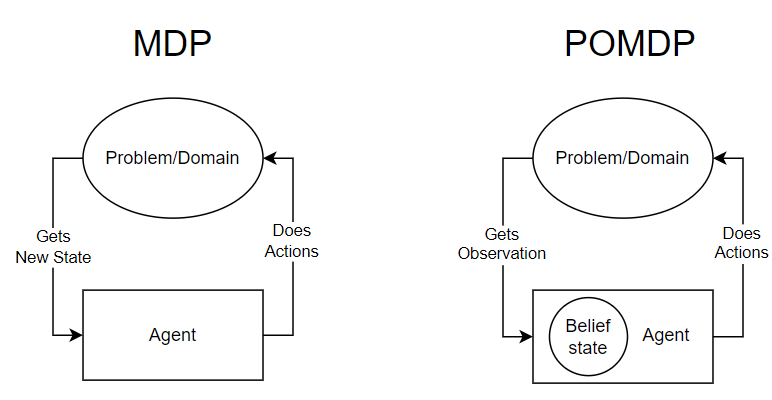
\includegraphics[width=0.8\textwidth]{images/MDP_POMDP_comparison.png}
    \caption{Differences between MDP and POMDP.}
    \label{fig:MDP_POMDP}
\end{figure}

A \gls{POMDP} extends the \gls{MDP} framework by explicitly acknowledging this imperfect perception. It is typically defined by a tuple \((S, A, P, R, \Omega, O, \gamma)\), where \(S\), \(A\), \(P\), \(R\), and \(\gamma\) are similar to their \gls{MDP} counterparts. The new components are the observation space \(\Omega\), a set of all possible observations \(o \in \Omega\) that the agent can receive from the environment, and the Observation Probability Function \(O(o | s', a)\), which defines the probability of the agent receiving observation \(o\) given that the environment has transitioned to the true state \(s'\) after the agent took action \(a\) in the previous (hidden) state.

In a \gls{POMDP}, since the true state \(s\) is not directly known, the agent cannot base its decisions directly on \(s\). Instead, the agent must operate based on the history of its actions and the observations it has received. To make optimal decisions, an agent in a POMDP often needs to maintain a belief state: 
\[b(s_t) = Pr(s_t | o_t, a_{t-1}, o_{t-1}, ..., a_0, o_0)\] 
which is a probability distribution over the set of all possible true states \(S\), representing the belief of the agent about the current true state \(s_t\) given the entire history of past actions and observations up to time \(t\). This belief state can be updated recursively using Bayes' rule: 
\[b_t(s') \propto  O(o_t | s', a_{t-1}) \Sigma_{s \in S} P(s' | s, a_{t-1}) b_{t-1}(s)\] 
The policy in a \gls{POMDP} thus becomes a mapping from belief states (or, more practically, from histories of observations) to actions: \(\pi(a | b)\) or \(\pi(a | h_t)\) where \(h_t = (o_0, a_0, ..., a_{t-1}, o_t)\) is the observation-action history. Finding an optimal policy in a \gls{POMDP} is significantly more challenging than in an \gls{MDP} because the agent must contend with uncertainty about the true state of the world and potentially infer it from a stream of partial information.

The problem of stock trading, which is the focus of this thesis, serves as a quintessential example of a \gls{POMDP}. An \gls{RL} agent attempting to trade stocks does not have access to the complete, true state of the financial market. Factors such as the aggregate sentiment of all market participants, the undisclosed intentions and order books of other traders, unreleased material news, and the true "fair value" of assets remain largely hidden. The agent instead receives observations, such as historical price and volume data, technical indicators, and, in the context of this work, signals derived from \gls{LLM} analyzing news articles, financial reports, and social media. 

\section{Soft Actor-Critic}
\label{sec:sac}
In \gls{RL} field, \gls{SAC} stands as a state-of-the-art algorithm, particularly recognized for its efficacy and stability in continuous action spaces, though adaptable to discrete ones as well.What distinguishes \gls{SAC} and contributes significantly to its robust performance is its core principle of maximum entropy reinforcement learning. Instead of solely aiming to maximize the conventional expected cumulative reward, \(\mathbb{E}_\pi[\Sigma_{t=0}^T \gamma^t R(s_t, a_t)]\), \gls{SAC} seeks to find a policy that also maximizes its own entropy at each step.

The inclusion of an entropy term in the objective function profoundly impacts the learning dynamics and the nature of the learned policy. The augmented \gls{SAC} objective function is expressed as:
\[J(\pi) = \mathbb{E}_{s_t \sim \rho_\pi, a_t \sim \pi(\cdot|s_t)} [R(s_t, a_t) + \alpha H(\pi(\cdot|s_t))]\]
Here, \(s_t\) are states (or, in a \gls{POMDP} context, history-derived observation representations) visited under policy \(\pi\), \(a_t\) are actions sampled from \(\pi(\cdot|s_t)\), \(R(s_t, a_t)\) is the immediate reward, and the entropy of the policy \(\pi\) in state \(s_t\) is:
\[H(\pi(\cdot|s_t)) = \mathbb{E}_{a_t \sim \pi(\cdot|s_t)}[-log \pi(a_t|s_t)]\] 
The temperature parameter \(\alpha > 0\), serves as a crucial trade-off coefficient, determining the relative importance of the entropy bonus compared to the extrinsic reward. A higher \(\alpha\) encourages more stochastic, exploratory behavior by pushing the policy towards a more uniform distribution over actions, while a lower \(\alpha\) shifts the focus more towards exploiting known good actions to maximize rewards. This entropy maximization offers several key advantages: it intrinsically promotes exploration, which is vital in complex environments with sparse rewards or deceptive local optima; it leads to policies that tend to be more robust to perturbations as they are less committed to a single, deterministic path; and it can accelerate learning by preventing premature convergence to suboptimal strategies.

To implement this maximum entropy objective, \gls{SAC} employs a sophisticated architecture, typically realized using neural networks for function approximation, which comprises several primary, interconnected components.

First is the Actor, or Policy Network, denoted as \(\pi_\phi(a|s)\) and parameterized by \(\phi\). This network is responsible for learning the agent's behavior. It takes the current state \(s\) as input and outputs the parameters of a probability distribution over the action space. For continuous actions, this is commonly a Gaussian distribution, where the network outputs the mean \(\mu_\phi(s)\) and standard deviation \(\sigma_\phi(s)\). Actions are then stochastically sampled from this distribution during interaction with the environment. The  learning objective of the actor is to choose actions that not only lead to high expected future rewards (as estimated by the critic) but also maintain high policy entropy. To enable gradient-based optimization through the stochastic sampling process, especially in continuous action spaces, \gls{SAC} utilizes the reparameterization trick. This involves expressing the sampled action \(a_t\) as a deterministic function of the policy parameters and an independent noise variable \(\epsilon\): 
\[a_t = \mu_\phi(s_t) + \sigma_\phi(s_t) \cdot \epsilon, \epsilon \sim \mathcal{N}(0,I)\]

Second, the Critic component in \gls{SAC} learns one or, more commonly, two Soft Q-Value Networks, \(Q_\theta(s, a)\), parameterized by \(\theta\). These networks learn to estimate the expected sum of future rewards and future entropy bonuses, if the agent starts in state \(s\), takes action \(a\), and subsequently follows the current policy \(\pi\) thereafter. This is known as the soft Q-value. The learning of these Q-functions is guided by a modified Bellman equation that incorporates the entropy term. The target for the soft Q-function is:
\[y(r, s') = r + \gamma(\mathbb{E}_{a' \sim \pi(\cdot|s')} [Q_{target}(s', a')] - \alpha \log \pi(a'|s'))\] 
The Q-networks are then trained by minimizing the soft Bellman residual, typically the squared error: 
\[L_Q(\theta) = \mathbb{E}_{(s,a,r,s') \sim \mathcal{D}} [(Q_\theta(s,a) - y(r,s'))^2]\]
where \(\mathcal{D}\) is the replay buffer. To combat the overestimation bias common in actor-critic methods, \gls{SAC} often implements the Clipped Double Q-learning technique. This involves learning two independent Q-networks (\(Q_{\theta_1}\) and \(Q_{\theta_2}\)) and using the minimum of their predictions when constructing the target value in the Bellman updates:
\[y(r, s') = r + \gamma(\mathbb{E}_{a' \sim \pi(\cdot|s')} [\min(Q_{target,1}(s', a'), Q_{target,2}(s', a'))] - \alpha \log \pi(a'|s'))\]
This conservative approach helps to mitigate positive bias and generally leads to more stable and reliable value estimates.

Third, to further enhance stability in the learning of the Q-functions, \gls{SAC} utilizes Target Q-Networks (\(Q_{\theta'_1}\) and \(Q_{\theta'_2}\), or \(Q_{target,1}\) and \(Q_{target,2}\) in the equation above) for the critic. These are separate networks whose parameters are periodically or slowly updated copies of the parameter of the main Q-networks. A common update rule is Polyak averaging: 
\[\theta'_i \leftarrow \tau\theta_i + (1-\tau)\theta'_i, i=1,2\] 
where \(\tau\) is a small constant. By using these slowly changing target networks to calculate the target values in the Bellman equation, the learning process is less prone to oscillations and divergence.

Fourth, a distinctive feature of many \gls{SAC} implementations is the Automated Temperature Parameter \(\alpha\) Tuning. While \(\alpha\) can be set as a fixed hyperparameter, \gls{SAC} often benefits from making \(\alpha\) a learnable parameter. This allows the algorithm to dynamically adjust the emphasis on entropy throughout the learning process, adapting the exploration-exploitation balance. The objective for learning \(\alpha\) is typically to maintain the policy's entropy at a predefined target entropy level \(\mathcal{H}_{target}\) (often set heuristically, e.g., \(-\text{dim}(\mathcal{A})\), where \(\text{dim}(\mathcal{A})\) is the action space dimensionality). This is achieved by performing gradient descent on \(\alpha\) to minimize the objective:
\[L(\alpha) = \mathbb{E}_{a_t \sim \pi(\cdot|s_t)} [-\alpha (\log \pi(a_t|s_t) + \mathcal{H}_{target})]\]

In summary, this chapter formalizes our problem as a \gls{POMDP} in which a \gls{SAC} agent leverages both quantitative market features and \gls{LLM}‑derived sentiment signals, reviews the strengths and limitations of deep \gls{RL} approaches versus traditional portfolio methods and of modern \gls{LLM}‑based sentiment analysis versus lexicon‑based techniques, and details the theoretical underpinnings of \gls{MDP}s/\gls{POMDP}s and the entropy‑regularized \gls{SAC} algorithm that together provide the foundation for our \gls{LLM}‑augmented trading framework.


\newpage
\chapter{METHODOLOGY}
\documentclass[../main.tex]{subfiles}
\begin{document}

\section{Overview}

Phần này mô tả tổng quan giải pháp gồm những bước chính nào, hoạt động ra sao. Mục tiêu của phần này là cho người đọc một cái nhìn tổng thể về giải pháp. Để cho dễ hiểu thì nên có một biểu đồ mô tả luồng hoạt động của giải pháp đề xuất. 

\section{Tên của nội dung chi tiết thứ 1}
Tên của các chương này đặt theo nội dung mà sinh viên sẽ trình bày trong từng chương. 

Các chương tiếp theo mô tả chi tiết về các bước, các thuật toán trong giải pháp đề xuất. Có thể trình bày pseudocode cho từng bước. Chú ý, pseudocode chỉ có tác dụng làm chi tiết hoá giải thuật chứ không thay thế được phần thuyết minh về giải thuật. Đối với những chi tiết kỹ thuật khó hiểu nên có các hình minh hoạ để người đọc dễ hiểu. Mỗi một thuật toán/bước thực hiện nên tách ra thành một chương. 

\section{Tên của nội dung chi tiết thứ 2}


\end{document}

\newpage
\chapter{THEORETICAL ANALYSIS}
\textcolor{red}{Chú ý: Chương này là không bắt buộc. Nếu nghiên cứu chỉ có đánh giá thực nghiệm mà không có phần thích lý thuyết thì sinh viên không cần trình bày chương này.} 

\section{Tên của kết quả phân tích số 1}

Nếu đồ án có phần phân tích lý thuyết thì sinh viên trình bày ở chương này. 

Kết quả lý thuyết có thể là phần tính toán về độ phức tạp tính toán của thuật toán hoặc chứng minh về tỉ số hiệu năng, \ldots

Nếu đồ án không có phần phân tích lý thuyết thì sinh viên không cần viết chương này. 

\section{Tên của kết quả phân tích số 2}


\newpage
\chapter{NUMERICAL RESULTS}
\documentclass[../main.tex]{subfiles}
\begin{document}

\textcolor{red}{Chú ý: Chương này là không bắt buộc. Nếu nghiên cứu chỉ có phân tích lý thuyết mà không có thực nghiệm thì sinh viên không cần trình bày chương này }

\section{Evaluation Parameters}

Sinh viên trình bày cụ thể về các tham số dùng trong đánh giá 

\section{Simulation Method}

Sinh viên trình bày chi tiết cách thức tiến hành thí nghiệm, ví dụ: các baseline chọn để so sánh là gì? tại sao lại chọn các baseline đấy? Tiến hành bao nhiêu thí nghiệm? mỗi thí nghiệm được thực hiện bao nhiêu lần? Các tham số của thuật toán được chọn như thế nào? Kịch bản thí nghiệm được tạo ra sao? Dữ liệu xử lý thế nào? … Có thể chia  chương này thành các chương nhỏ hơn để tiện trình bày. 

\section{Tên của kết quả thí nghiệm 1}

Các chương tiếp theo sinh viên trình bày các kết quả thí nghiệm thu được. Mỗi kết quả nên cho vào một chương. Đối với mỗi kết quả thí nghiệm, cần trình bày các bảng biểu, đồ thị minh hoạ cho kết quả thí nghiệm. Sinh viên cần nêu nhận xét chi tiết về kết quả thí nghiệm, so sánh các phương pháp với nhau, giải thích tại sao kết quả lại như vậy. 

\section{Tên của kết quả thí nghiệm 2}

\end{document}

\newpage
\chapter{CONCLUSIONS}
\documentclass[../main.tex]{subfiles}
\begin{document}

\section{Summary}

Sinh viên nhắc lại các vấn đề mà đồ án đã giải quyết được, cũng như những vấn đề còn tồn đọng của đồ án.  

\section{Suggestion for Future Works }

Sinh viên đề xuất hướng phát triển trong tương lai (nếu có) .  

\end{document}

\printbibliography
\end{document}
